% Created by tikzDevice version 0.12.6 on 2025-08-19 18:47:20
% !TEX encoding = UTF-8 Unicode
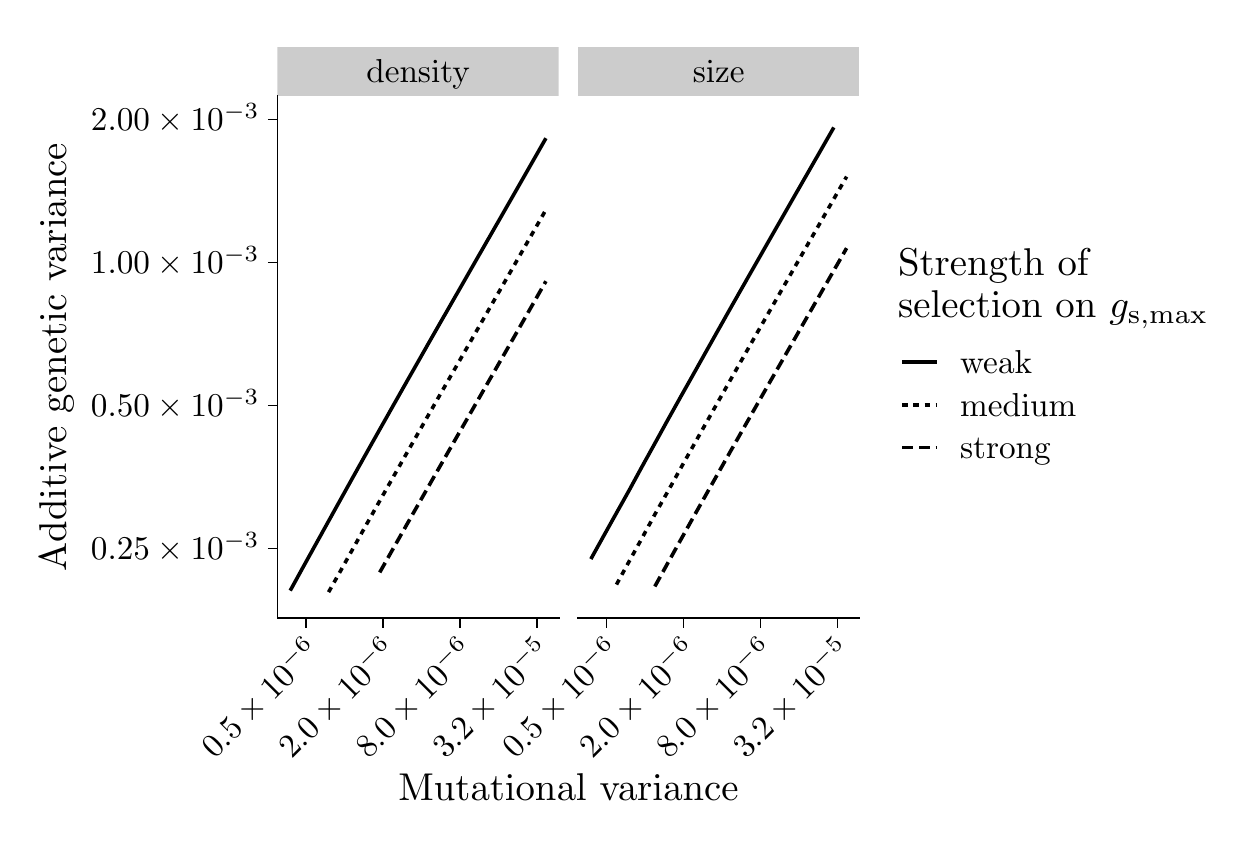
\begin{tikzpicture}[x=1pt,y=1pt]
\definecolor{fillColor}{RGB}{255,255,255}
\path[use as bounding box,fill=fillColor,fill opacity=0.00] (0,0) rectangle (433.62,289.08);
\begin{scope}
\path[clip] ( 90.25, 75.67) rectangle (191.89,264.48);
\definecolor{drawColor}{RGB}{0,0,0}

\path[draw=drawColor,line width= 1.3pt,line join=round] ( 94.87, 85.66) --
	( 99.49, 94.08) --
	(104.11,102.43) --
	(108.73,110.77) --
	(113.35,119.10) --
	(117.97,127.41) --
	(122.59,135.68) --
	(127.21,143.89) --
	(131.83,152.08) --
	(136.45,160.25) --
	(141.07,168.37) --
	(145.69,176.51) --
	(150.31,184.58) --
	(154.93,192.64) --
	(159.55,200.71) --
	(164.17,208.76) --
	(168.79,216.81) --
	(173.41,224.87) --
	(178.03,232.93) --
	(182.65,241.03) --
	(187.27,249.13);

\path[draw=drawColor,line width= 1.3pt,dash pattern=on 2pt off 2pt ,line join=round] (108.73, 85.11) --
	(113.35, 93.31) --
	(117.97,101.59) --
	(122.59,109.88) --
	(127.21,118.08) --
	(131.83,126.25) --
	(136.45,134.40) --
	(141.07,142.53) --
	(145.69,150.65) --
	(150.31,158.73) --
	(154.93,166.80) --
	(159.55,174.86) --
	(164.17,182.92) --
	(168.79,190.98) --
	(173.41,199.03) --
	(178.03,207.11) --
	(182.65,215.19) --
	(187.27,223.29);

\path[draw=drawColor,line width= 1.3pt,dash pattern=on 4pt off 2pt ,line join=round] (127.21, 92.24) --
	(131.83,100.42) --
	(136.45,108.56) --
	(141.07,116.69) --
	(145.69,124.80) --
	(150.31,132.90) --
	(154.93,140.99) --
	(159.55,149.02) --
	(164.17,157.08) --
	(168.79,165.15) --
	(173.41,173.20) --
	(178.03,181.27) --
	(182.65,189.36) --
	(187.27,197.46);
\end{scope}
\begin{scope}
\path[clip] (198.89, 75.67) rectangle (300.54,264.48);
\definecolor{drawColor}{RGB}{0,0,0}

\path[draw=drawColor,line width= 1.3pt,line join=round] (203.51, 97.07) --
	(208.13,105.41) --
	(212.76,113.72) --
	(217.38,121.97) --
	(222.00,130.48) --
	(226.62,138.83) --
	(231.24,147.23) --
	(235.86,155.51) --
	(240.48,163.72) --
	(245.10,171.97) --
	(249.72,180.18) --
	(254.34,188.38) --
	(258.96,196.50) --
	(263.58,204.61) --
	(268.20,212.70) --
	(272.82,220.78) --
	(277.44,228.85) --
	(282.06,236.90) --
	(286.68,244.96) --
	(291.30,253.02);

\path[draw=drawColor,line width= 1.3pt,dash pattern=on 2pt off 2pt ,line join=round] (212.76, 87.86) --
	(217.38, 96.30) --
	(222.00,104.65) --
	(226.62,113.17) --
	(231.24,121.34) --
	(235.86,129.68) --
	(240.48,137.92) --
	(245.10,146.14) --
	(249.72,154.34) --
	(254.34,162.51) --
	(258.96,170.67) --
	(263.58,178.80) --
	(268.20,186.86) --
	(272.82,194.94) --
	(277.44,203.01) --
	(282.06,211.08) --
	(286.68,219.12) --
	(291.30,227.19) --
	(295.92,235.25);

\path[draw=drawColor,line width= 1.3pt,dash pattern=on 4pt off 2pt ,line join=round] (226.62, 87.17) --
	(231.24, 95.50) --
	(235.86,103.80) --
	(240.48,112.08) --
	(245.10,120.29) --
	(249.72,128.49) --
	(254.34,136.67) --
	(258.96,144.81) --
	(263.58,152.94) --
	(268.20,161.05) --
	(272.82,169.10) --
	(277.44,177.17) --
	(282.06,185.24) --
	(286.68,193.28) --
	(291.30,201.34) --
	(295.92,209.41);
\end{scope}
\begin{scope}
\path[clip] ( 90.25,264.48) rectangle (191.89,282.08);
\definecolor{fillColor}{gray}{0.80}

\path[fill=fillColor] ( 90.25,264.48) rectangle (191.89,282.08);
\definecolor{drawColor}{RGB}{0,0,0}

\node[text=drawColor,anchor=base,inner sep=0pt, outer sep=0pt, scale=  1.20] at (141.07,269.15) {density};
\end{scope}
\begin{scope}
\path[clip] (198.89,264.48) rectangle (300.54,282.08);
\definecolor{fillColor}{gray}{0.80}

\path[fill=fillColor] (198.89,264.48) rectangle (300.54,282.08);
\definecolor{drawColor}{RGB}{0,0,0}

\node[text=drawColor,anchor=base,inner sep=0pt, outer sep=0pt, scale=  1.20] at (249.72,269.15) {size};
\end{scope}
\begin{scope}
\path[clip] (  0.00,  0.00) rectangle (433.62,289.08);
\definecolor{drawColor}{RGB}{0,0,0}

\path[draw=drawColor,line width= 0.6pt,line join=round,line cap=rect] ( 90.25, 75.67) --
	(191.89, 75.67);
\end{scope}
\begin{scope}
\path[clip] (  0.00,  0.00) rectangle (433.62,289.08);
\definecolor{drawColor}{RGB}{0,0,0}

\path[draw=drawColor,line width= 0.6pt,line join=round] (100.52, 72.17) --
	(100.52, 75.67);

\path[draw=drawColor,line width= 0.6pt,line join=round] (128.33, 72.17) --
	(128.33, 75.67);

\path[draw=drawColor,line width= 0.6pt,line join=round] (156.15, 72.17) --
	(156.15, 75.67);

\path[draw=drawColor,line width= 0.6pt,line join=round] (183.97, 72.17) --
	(183.97, 75.67);
\end{scope}
\begin{scope}
\path[clip] (  0.00,  0.00) rectangle (433.62,289.08);
\definecolor{drawColor}{RGB}{0,0,0}

\node[text=drawColor,rotate= 45.00,anchor=base east,inner sep=0pt, outer sep=0pt, scale=  1.20] at (106.36, 63.32) {$0.5 \times 10^{-6}$};

\node[text=drawColor,rotate= 45.00,anchor=base east,inner sep=0pt, outer sep=0pt, scale=  1.20] at (134.18, 63.32) {$2.0 \times 10^{-6}$};

\node[text=drawColor,rotate= 45.00,anchor=base east,inner sep=0pt, outer sep=0pt, scale=  1.20] at (162.00, 63.32) {$8.0 \times 10^{-6}$};

\node[text=drawColor,rotate= 45.00,anchor=base east,inner sep=0pt, outer sep=0pt, scale=  1.20] at (189.81, 63.32) {$3.2 \times 10^{-5}$};
\end{scope}
\begin{scope}
\path[clip] (  0.00,  0.00) rectangle (433.62,289.08);
\definecolor{drawColor}{RGB}{0,0,0}

\path[draw=drawColor,line width= 0.6pt,line join=round,line cap=rect] (198.89, 75.67) --
	(300.54, 75.67);
\end{scope}
\begin{scope}
\path[clip] (  0.00,  0.00) rectangle (433.62,289.08);
\definecolor{drawColor}{RGB}{0,0,0}

\path[draw=drawColor,line width= 0.6pt,line join=round] (209.16, 72.17) --
	(209.16, 75.67);

\path[draw=drawColor,line width= 0.6pt,line join=round] (236.98, 72.17) --
	(236.98, 75.67);

\path[draw=drawColor,line width= 0.6pt,line join=round] (264.80, 72.17) --
	(264.80, 75.67);

\path[draw=drawColor,line width= 0.6pt,line join=round] (292.62, 72.17) --
	(292.62, 75.67);
\end{scope}
\begin{scope}
\path[clip] (  0.00,  0.00) rectangle (433.62,289.08);
\definecolor{drawColor}{RGB}{0,0,0}

\node[text=drawColor,rotate= 45.00,anchor=base east,inner sep=0pt, outer sep=0pt, scale=  1.20] at (215.01, 63.32) {$0.5 \times 10^{-6}$};

\node[text=drawColor,rotate= 45.00,anchor=base east,inner sep=0pt, outer sep=0pt, scale=  1.20] at (242.83, 63.32) {$2.0 \times 10^{-6}$};

\node[text=drawColor,rotate= 45.00,anchor=base east,inner sep=0pt, outer sep=0pt, scale=  1.20] at (270.64, 63.32) {$8.0 \times 10^{-6}$};

\node[text=drawColor,rotate= 45.00,anchor=base east,inner sep=0pt, outer sep=0pt, scale=  1.20] at (298.46, 63.32) {$3.2 \times 10^{-5}$};
\end{scope}
\begin{scope}
\path[clip] (  0.00,  0.00) rectangle (433.62,289.08);
\definecolor{drawColor}{RGB}{0,0,0}

\path[draw=drawColor,line width= 0.6pt,line join=round,line cap=rect] ( 90.25, 75.67) --
	( 90.25,264.48);
\end{scope}
\begin{scope}
\path[clip] (  0.00,  0.00) rectangle (433.62,289.08);
\definecolor{drawColor}{RGB}{0,0,0}

\node[text=drawColor,anchor=base east,inner sep=0pt, outer sep=0pt, scale=  1.20] at ( 83.75, 96.75) {$0.25 \times 10^{-3}$};

\node[text=drawColor,anchor=base east,inner sep=0pt, outer sep=0pt, scale=  1.20] at ( 83.75,148.42) {$0.50 \times 10^{-3}$};

\node[text=drawColor,anchor=base east,inner sep=0pt, outer sep=0pt, scale=  1.20] at ( 83.75,200.10) {$1.00 \times 10^{-3}$};

\node[text=drawColor,anchor=base east,inner sep=0pt, outer sep=0pt, scale=  1.20] at ( 83.75,251.77) {$2.00 \times 10^{-3}$};
\end{scope}
\begin{scope}
\path[clip] (  0.00,  0.00) rectangle (433.62,289.08);
\definecolor{drawColor}{RGB}{0,0,0}

\path[draw=drawColor,line width= 0.6pt,line join=round] ( 86.75,100.88) --
	( 90.25,100.88);

\path[draw=drawColor,line width= 0.6pt,line join=round] ( 86.75,152.56) --
	( 90.25,152.56);

\path[draw=drawColor,line width= 0.6pt,line join=round] ( 86.75,204.23) --
	( 90.25,204.23);

\path[draw=drawColor,line width= 0.6pt,line join=round] ( 86.75,255.90) --
	( 90.25,255.90);
\end{scope}
\begin{scope}
\path[clip] (  0.00,  0.00) rectangle (433.62,289.08);
\definecolor{drawColor}{RGB}{0,0,0}

\node[text=drawColor,anchor=base,inner sep=0pt, outer sep=0pt, scale=  1.40] at (195.39,  9.72) {Mutational variance};
\end{scope}
\begin{scope}
\path[clip] (  0.00,  0.00) rectangle (433.62,289.08);
\definecolor{drawColor}{RGB}{0,0,0}

\node[text=drawColor,rotate= 90.00,anchor=base,inner sep=0pt, outer sep=0pt, scale=  1.40] at ( 13.92,170.07) {Additive genetic variance};
\end{scope}
\begin{scope}
\path[clip] (  0.00,  0.00) rectangle (433.62,289.08);
\definecolor{drawColor}{RGB}{0,0,0}

\node[text=drawColor,anchor=base west,inner sep=0pt, outer sep=0pt, scale=  1.40] at (314.54,199.41) {Strength of};

\node[text=drawColor,anchor=base west,inner sep=0pt, outer sep=0pt, scale=  1.40] at (314.54,184.29) {selection on $g_\mathrm{s,max}$};
\end{scope}
\begin{scope}
\path[clip] (  0.00,  0.00) rectangle (433.62,289.08);
\definecolor{drawColor}{RGB}{0,0,0}

\path[draw=drawColor,line width= 1.3pt,line join=round] (316.08,168.23) -- (328.40,168.23);
\end{scope}
\begin{scope}
\path[clip] (  0.00,  0.00) rectangle (433.62,289.08);
\definecolor{drawColor}{RGB}{0,0,0}

\path[draw=drawColor,line width= 1.3pt,dash pattern=on 2pt off 2pt ,line join=round] (316.08,152.83) -- (328.40,152.83);
\end{scope}
\begin{scope}
\path[clip] (  0.00,  0.00) rectangle (433.62,289.08);
\definecolor{drawColor}{RGB}{0,0,0}

\path[draw=drawColor,line width= 1.3pt,dash pattern=on 4pt off 2pt ,line join=round] (316.08,137.43) -- (328.40,137.43);
\end{scope}
\begin{scope}
\path[clip] (  0.00,  0.00) rectangle (433.62,289.08);
\definecolor{drawColor}{RGB}{0,0,0}

\node[text=drawColor,anchor=base west,inner sep=0pt, outer sep=0pt, scale=  1.20] at (336.94,164.10) {weak};
\end{scope}
\begin{scope}
\path[clip] (  0.00,  0.00) rectangle (433.62,289.08);
\definecolor{drawColor}{RGB}{0,0,0}

\node[text=drawColor,anchor=base west,inner sep=0pt, outer sep=0pt, scale=  1.20] at (336.94,148.70) {medium};
\end{scope}
\begin{scope}
\path[clip] (  0.00,  0.00) rectangle (433.62,289.08);
\definecolor{drawColor}{RGB}{0,0,0}

\node[text=drawColor,anchor=base west,inner sep=0pt, outer sep=0pt, scale=  1.20] at (336.94,133.30) {strong};
\end{scope}
\end{tikzpicture}
